\subsection{Interaktionsdiagramme}\label{interaktionsdiagramme}
Im folgenden Kapitel zeigen wir die wichtigsten Interaktionsdiagramme unseres Backend und der Frontend-Applikation auf.

\subsubsection{Backend}\label{backend}

\subsubsubsection{Tour starten}
Bei dem Prozess ``Tour starten'' im Backend wird zuerst überprüft, dass der angegebene Benutzer nicht bereits eine gestartet Tour hat. Anschliessend wird die angegebene Tour als gestartet markiert. Von dieser gestarteten Tour werden Informationen aus der Datenbank ausgelesen und auch die Route zum ersten POI berechnet. Die Informationen zum POI sowie auch die Route, werden an den Aufrufer zurückgegeben.

\begin{figure}
  \centering
  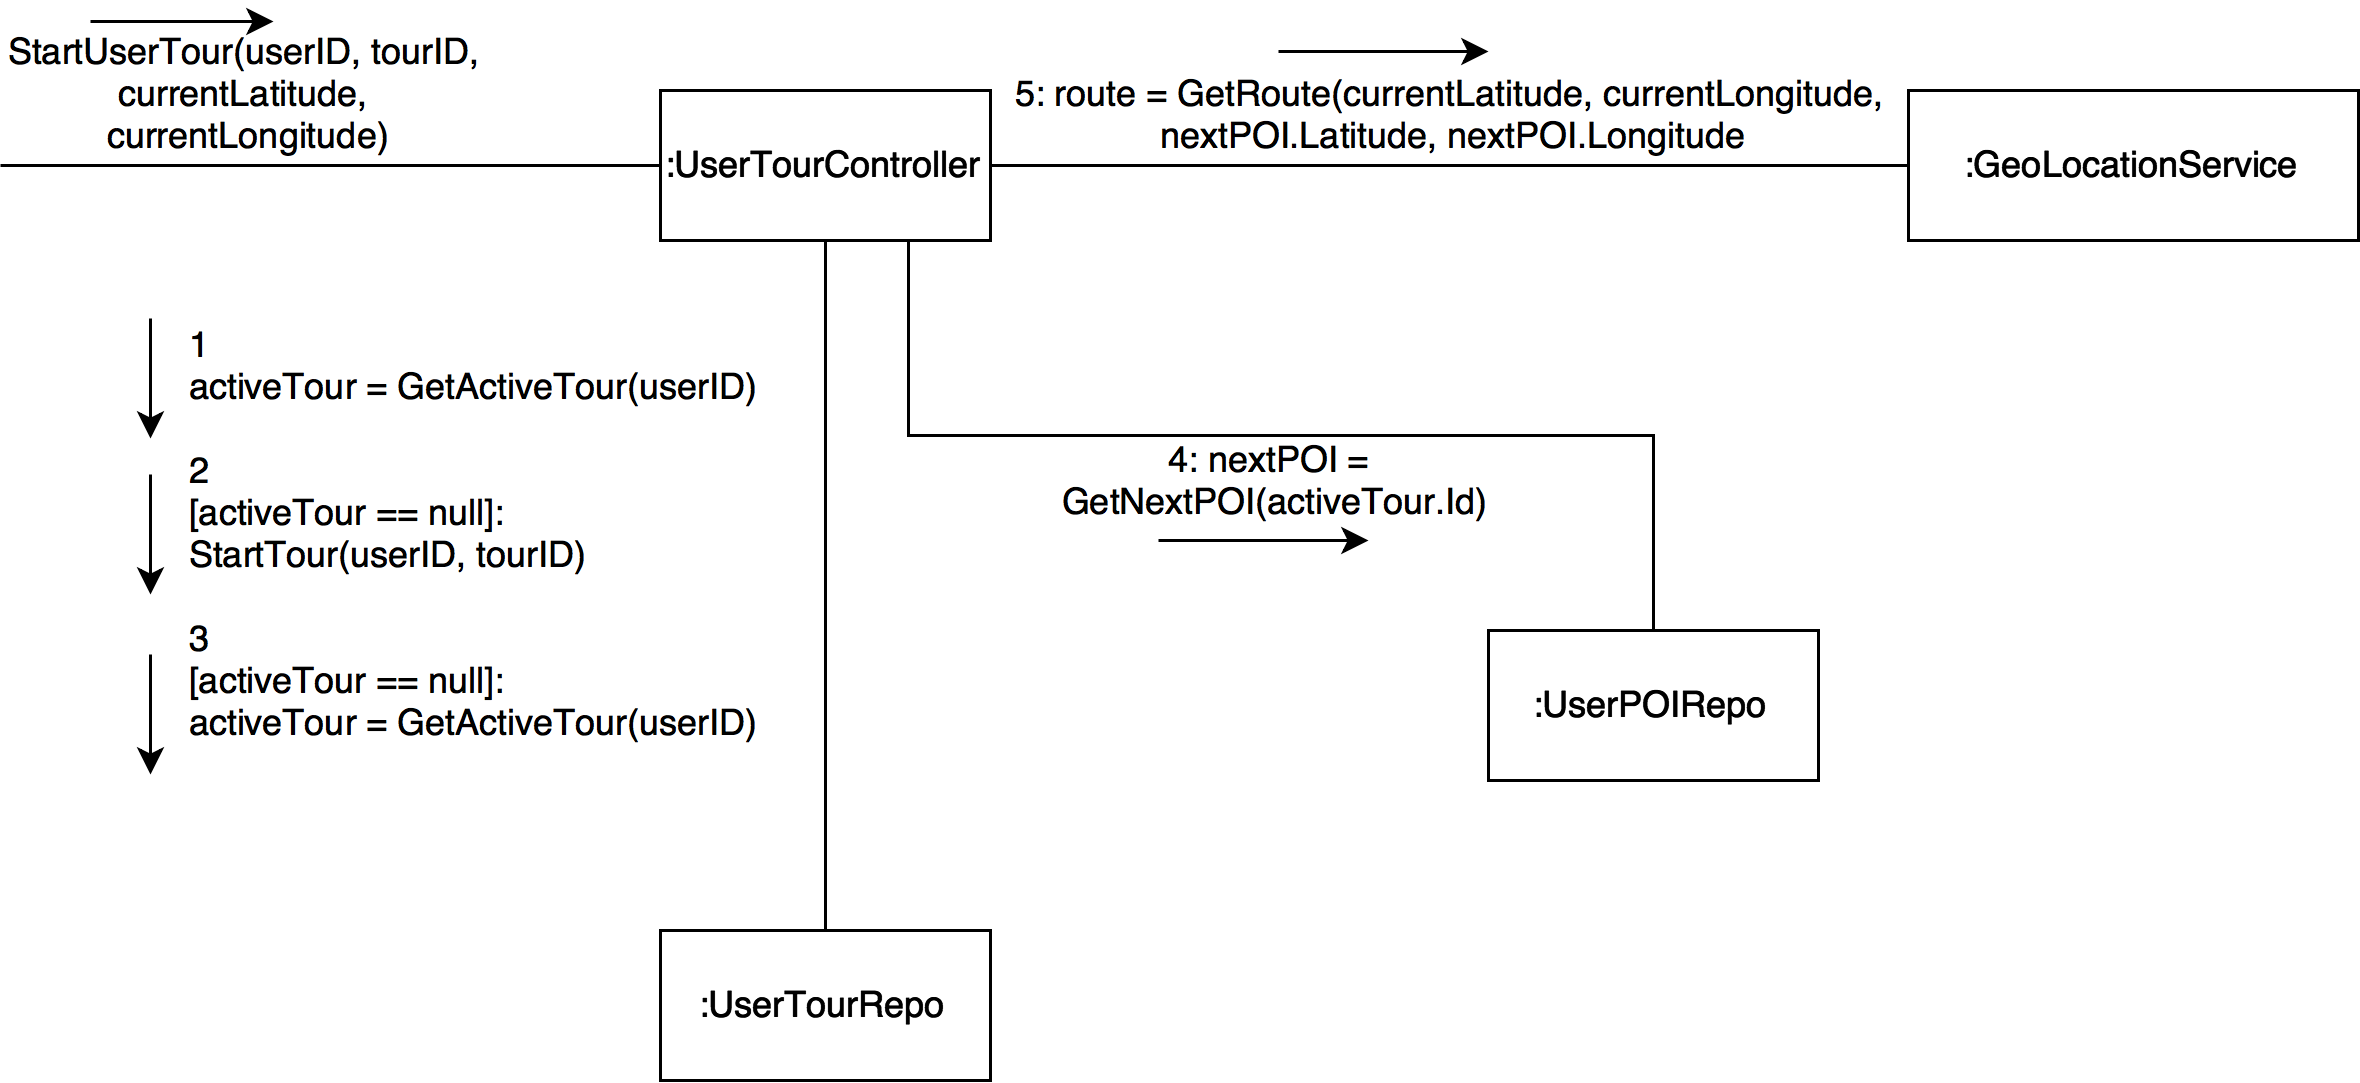
\includegraphics[height=5cm]{Kommunikationsdiagramm_StartTour}
  \caption{Kommunikationsdiagramm Tour starten}
\end{figure}

\subsubsubsection{Route zu POI}
Im Ablauf ``Route zu POI'' wird zuerst die aktuelle Tour des angegebenen Touristen aus der
Datenbank ausgelesen. Anhand dieser Tour wird anschliessend herausgefunden, welches der nächste
Besichtigungspunkt (POI) ist und aufgrund der aktuellen Position die Route zum nächsten
POI mittels Google-Maps API berechnet und zurück gegeben.

\begin{figure}
  \centering
  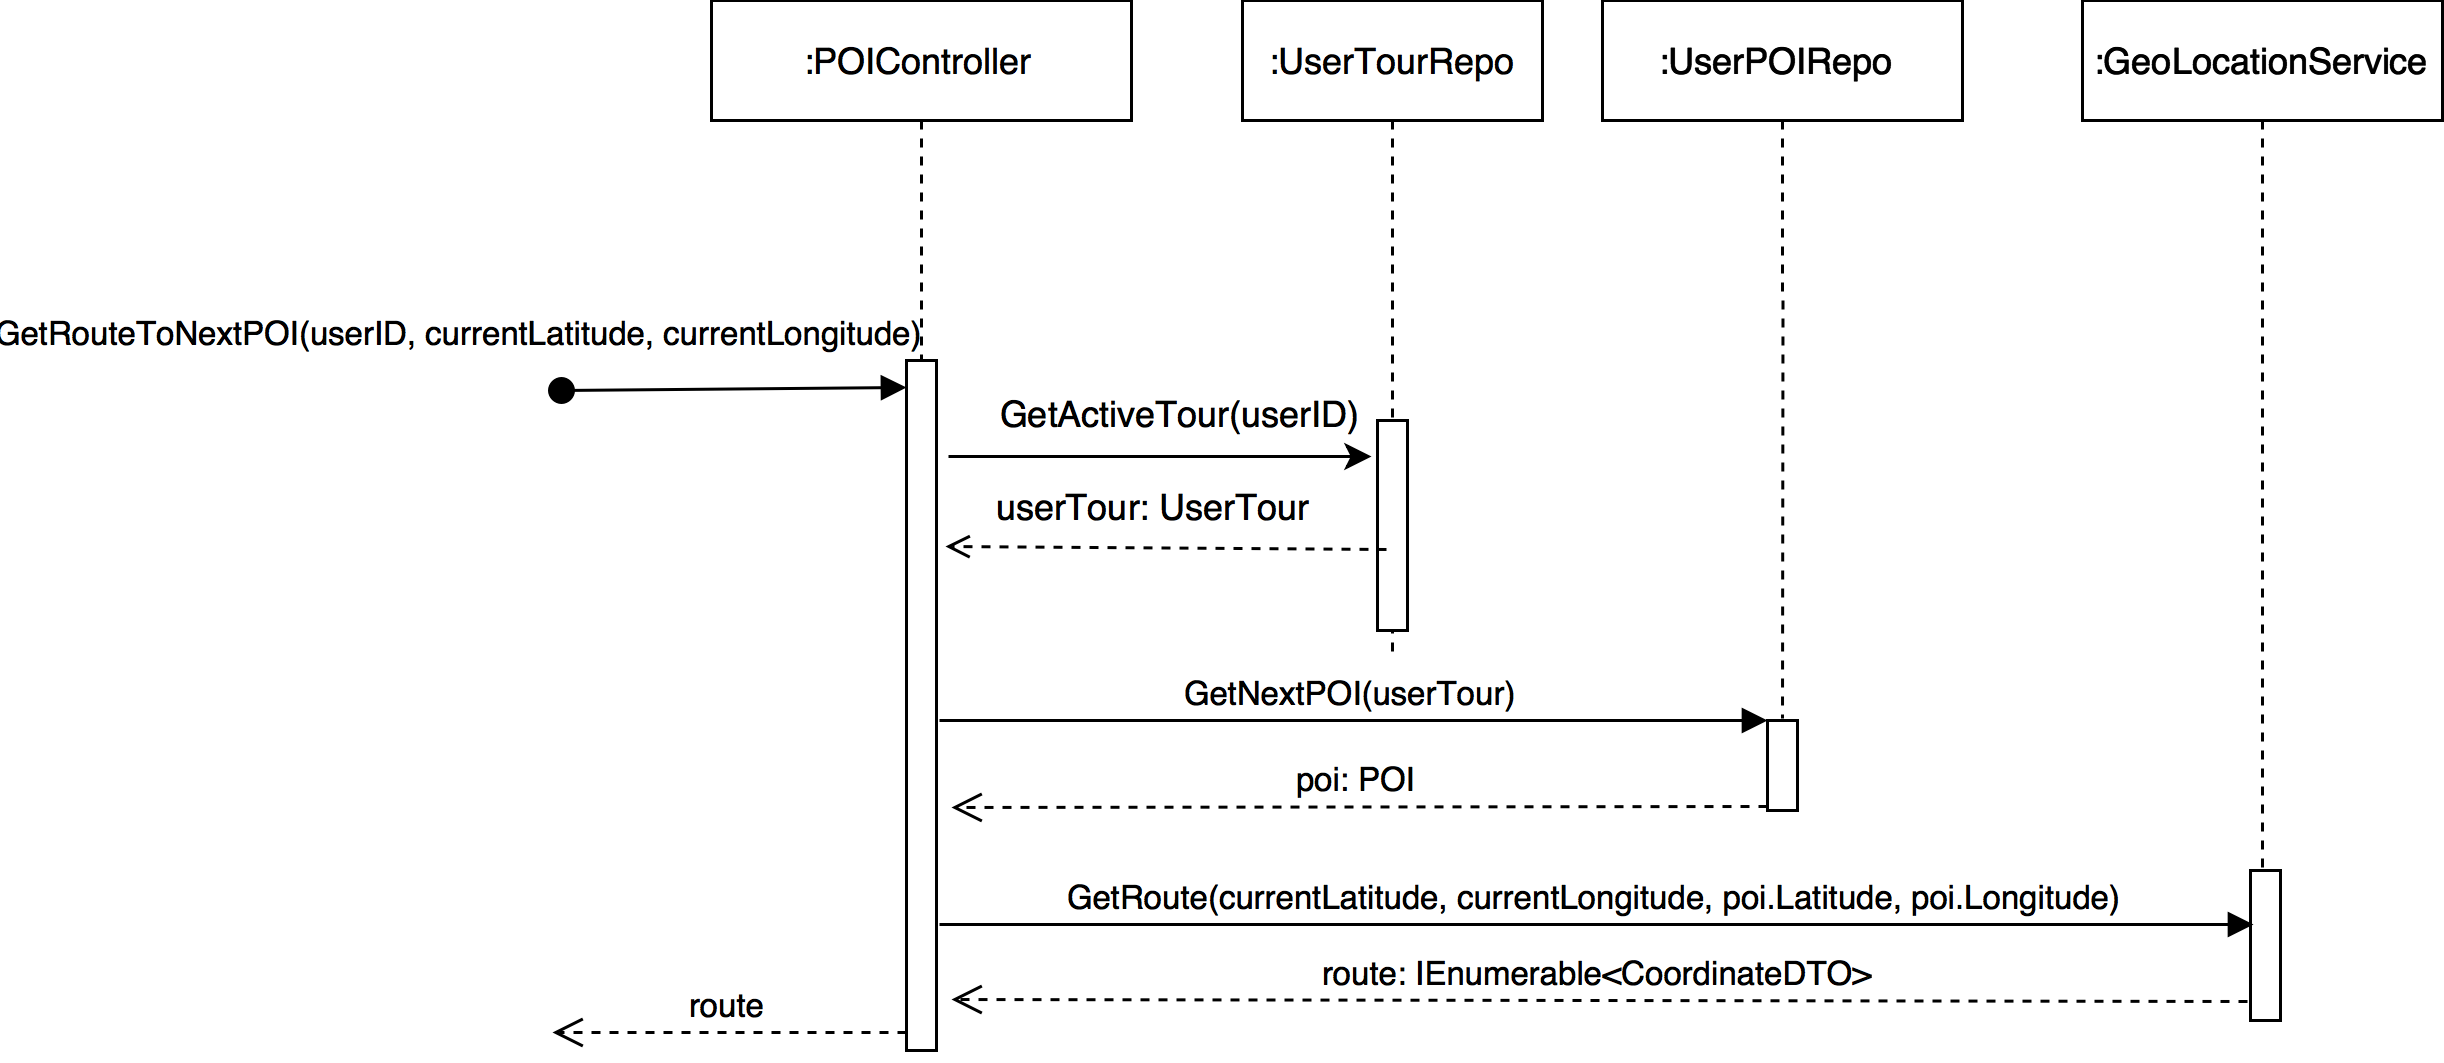
\includegraphics[height=6cm]{Sequenzdiagramm_GetRouteToPoi}
  \caption{Sequenzdiagramm Route zu POI}
\end{figure}

\subsubsection{Frontend}\label{frontend}
\subsubsubsection{Tour Liste anzeigen}\label{frontend-listactivity}
Dieser Ablauf zeigt den Prozess wie die Liste der verfügbaren Touren in der Applikation
angezeigt wird. Über den \textbf{RequestQueuer} werden asynchron die Touren vom Backend geladen.
Der \textbf{RequestQueuer} führt bei erfolgreicher Serverantwort das Callback aus, welches
wiederum die Touren in der View setzt und diese aktualisiert.

\begin{figure}
  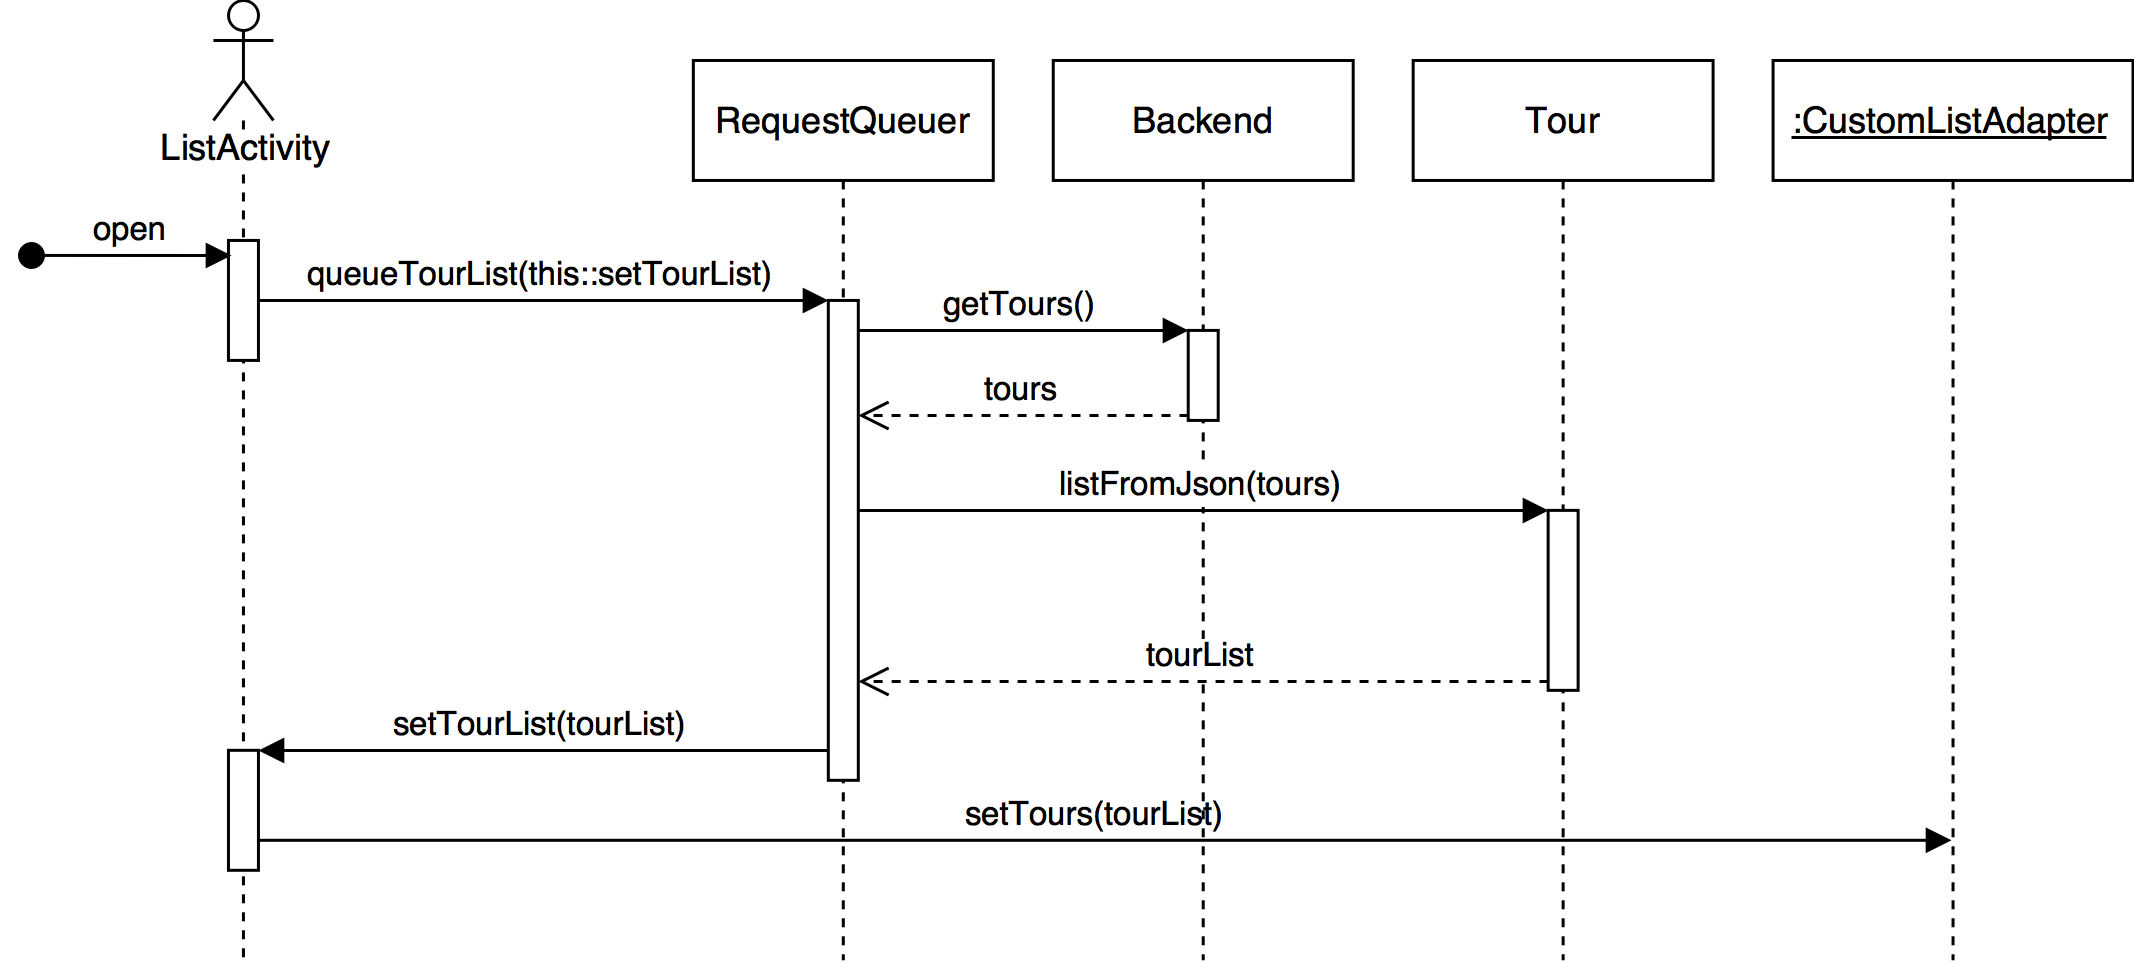
\includegraphics{Sequenzdiagramm_ListActivity}
  \caption{Sequenzdiagramm Tour Liste anzeigen}
\end{figure}

\subsubsubsection{Tour Details anzeigen}
Dieser Vorgang funktioniert ähnlich wie \fullref{frontend-listactivity}. Mittels
\textbf{RequestQueuer} werden alle POIs der ausgewählten Tour - welche der Activity übergeben
wurde - geladen, ebenfalls mittels Callback. Anschliessend werden die Daten der View
übergeben und die Karte gezeichnet.

\begin{figure}
  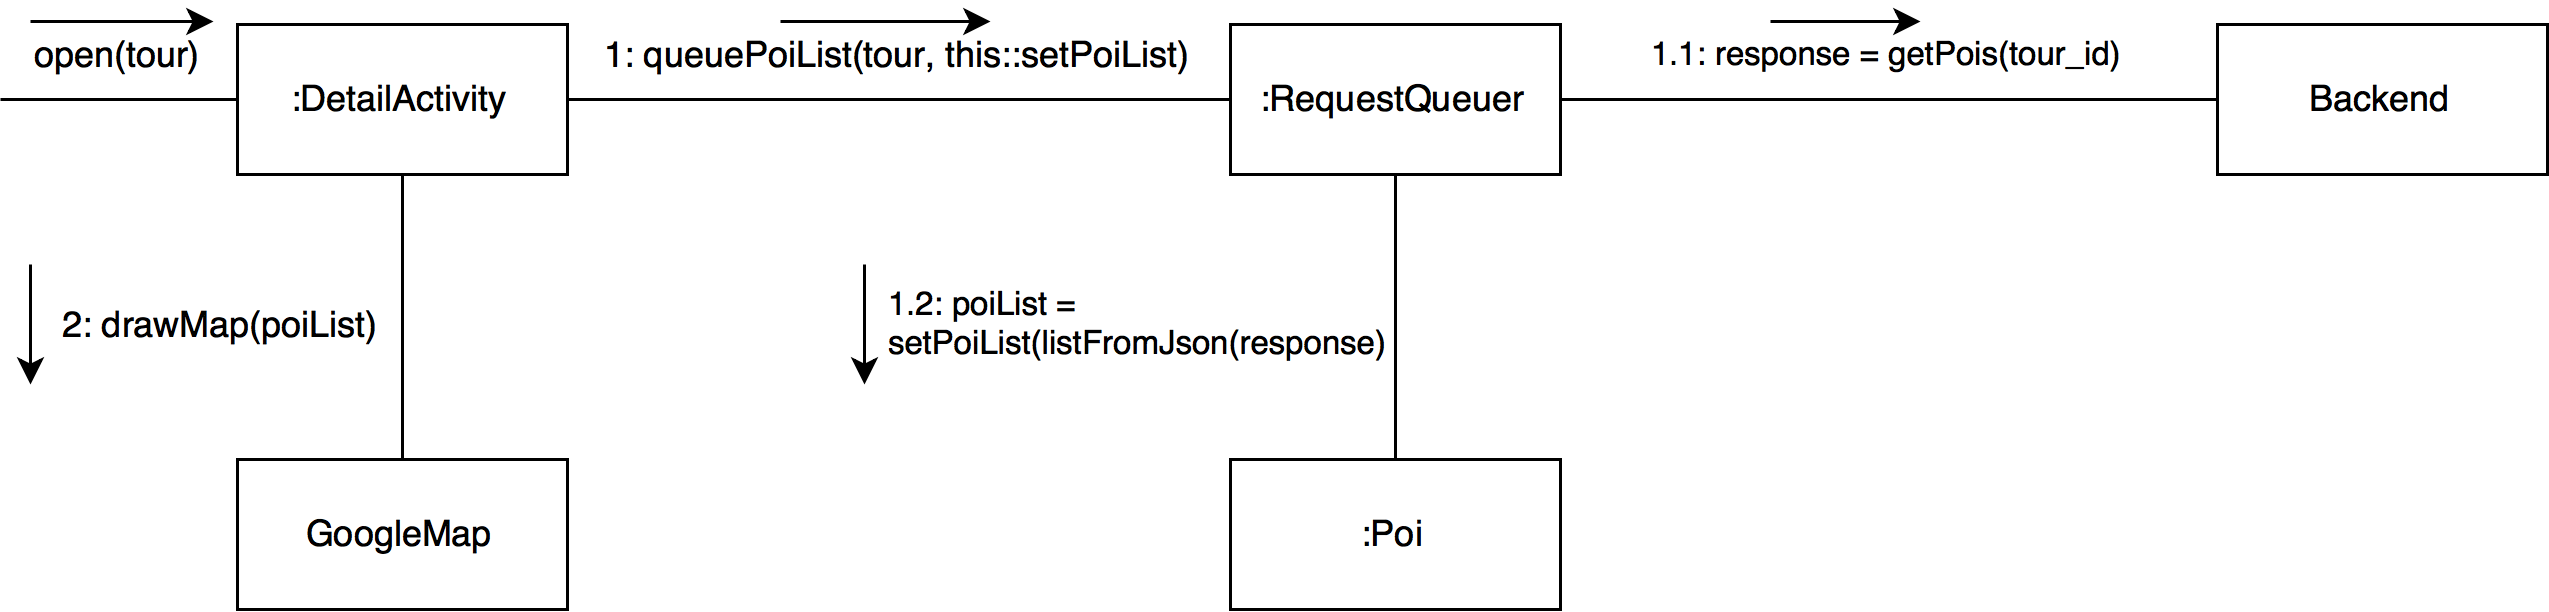
\includegraphics{Kommunikationsdiagramm_DetailActivity}
  \caption{Kommunikationsdiagramm Tour Details anzeigen}
\end{figure}

\newpage
\subsubsubsection{Checke, ob bei POI angekommen}
Das Diagram zeigt den wiederkehrenden Prozess wobei überprüft wird, ob der Tourist beim
ausgewählten POI angekommen ist. Der Google Maps Service ruft herzu bei der Veränderung
der Position eine Funktion auf. Diese benutzt den \textbf{RequestQueuer} um die Position
auf dem Backend zu überprüfen.

\begin{figure}
  \includegraphics{Sequenzdiagramm_IsNearPoi}
  \caption{Sequenzdiagramm Check ob bei POI angekommen}
\end{figure}

\newpage
\subsubsubsection{Foto aufnehmen}
Mit dem Ablauf ``Foto aufnehmen'' wird aufgezeigt wie ein Foto mit der Gerätekamera
aufgenommen wird und diese Anschliessend zur Tour abgelegt wird.

\begin{figure}
  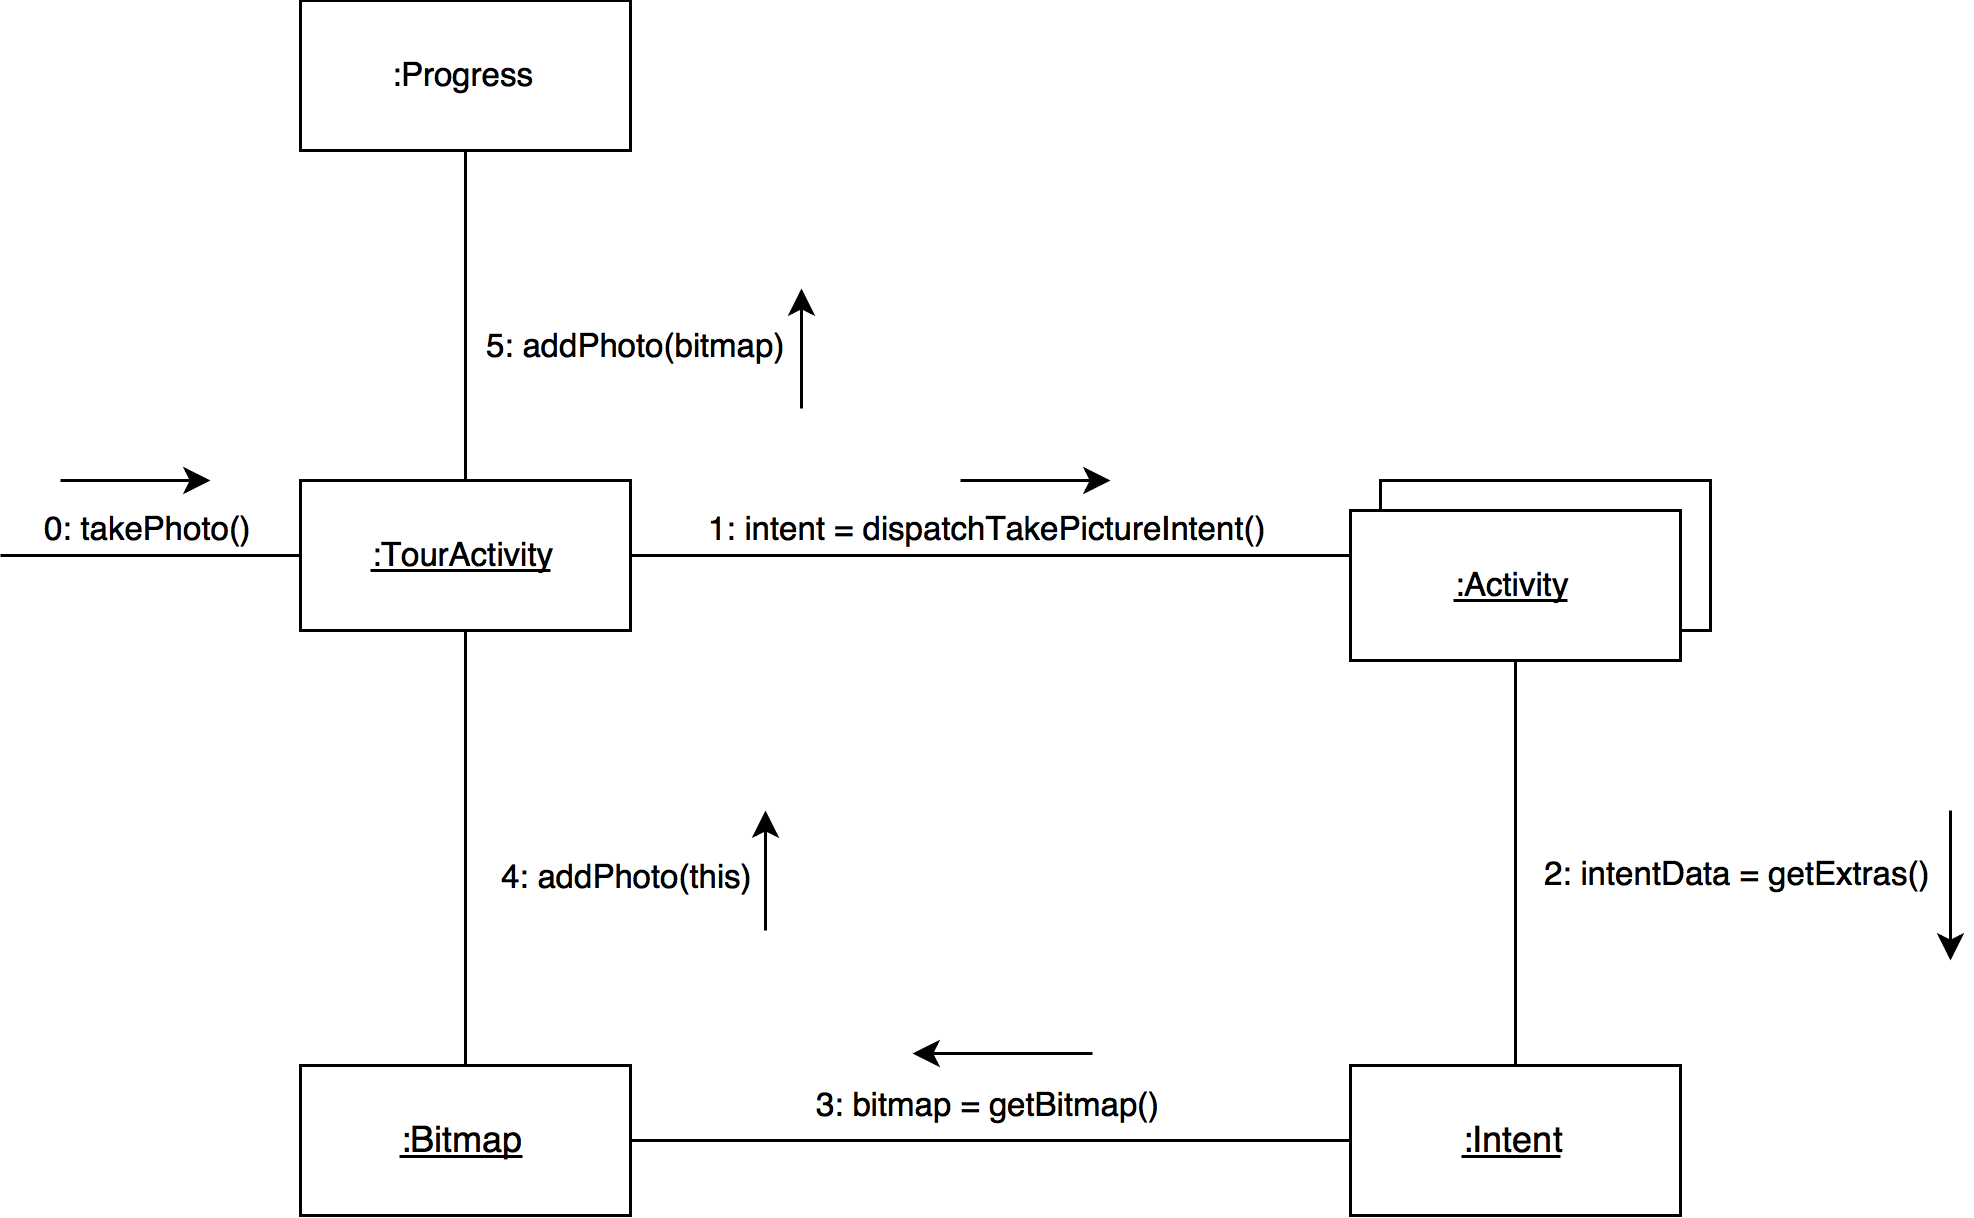
\includegraphics{Kommunikationsdiagramm_TakePhoto}
  \caption{Kommunikationsdiagramm Foto aufnehmen}
\end{figure}

\subsubsubsection{Summary anzeigen}
Dieser Vorgang zeigt den Abschluss einer Tour auf, wobei eine Übersicht der Tourdaten
generiert und angezeigt wird.
\begin{figure}
  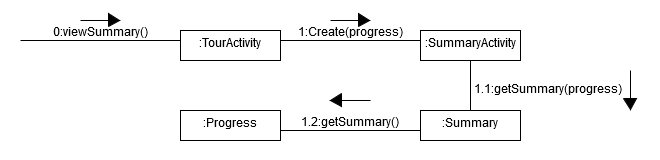
\includegraphics{Kommunikationsdiagramm_SummaryActivity}
  \caption{Kommunikationsdiagram Summary anzeigen}
\end{figure}
